\documentclass[11pt]{article}

% Change "review" to "final" to generate the final (sometimes called camera-ready) version.
% Change to "preprint" to generate a non-anonymous version with page numbers.
\usepackage[final]{acl}

% Standard package includes
\usepackage{times}
\usepackage{latexsym}

% For mathematical typesetting and \text command
\usepackage{amsmath}

% For customizing lists (enumerate, itemize)
\usepackage{enumitem}

% tu use algorithms 
\usepackage{algorithm}
\usepackage{algpseudocode}
\usepackage{xcolor}

% For proper rendering and hyphenation of words containing Latin characters (including in bib files)
\usepackage[T1]{fontenc}
% For Vietnamese characters
% \usepackage[T5]{fontenc}
% See https://www.latex-project.org/help/documentation/encguide.pdf for other character sets

% This assumes your files are encoded as UTF8
\usepackage[utf8]{inputenc}

% For cross-references with \cref command
\usepackage{cleveref}

% This is not strictly necessary, and may be commented out,
% but it will improve the layout of the manuscript,
% and will typically save some space.
\usepackage{microtype}

% This is also not strictly necessary, and may be commented out.
% However, it will improve the aesthetics of text in
% the typewriter font.
\usepackage{inconsolata}

%Including images in your LaTeX document requires adding
%additional package(s)
\usepackage{graphicx}
\usepackage{booktabs}
\usepackage{multirow}

% If the title and author information does not fit in the area allocated, uncomment the following
%
%\setlength\titlebox{<dim>}
%
% and set <dim> to something 5cm or larger.

\title{FastDetectGPT: Understanding Sampling-based Zero-shot AI-generated Text Detection}

\author{
  \textbf{Jose Garcia\textsuperscript{1}},
  \textbf{Krystof Bobek\textsuperscript{1}},
  \textbf{Mara Dragomir\textsuperscript{1}}, \\
  \textbf{Mahdi Rahimi\textsuperscript{1}},
  \textbf{Salvador Torpes\textsuperscript{1}}
\\
\\
  \textsuperscript{1}University of Amsterdam
\\
\\
  \textbf{Contact:} \{
    \texttt{jose.garcia.carrillo, krystof.bobek, mara.dragomir,} \\
    \texttt{mahdi.rahimi, salvador.baptista.torpes} \}
    \texttt{@student.uva.nl}
}

\begin{document}

\maketitle

\begin{abstract}
  DetectGPT introduced a sampling-based zero shot detector that exploits local curvature of the log likelihood surface to distinguish machine-generated from human written text. Fast DetectGPT later proposed a faster method that maintains strong performance with reduced computational cost. In this project we reproduce Fast DetectGPT as baselines with new source models (R1-8B, Phi-2, Mistral-7B, GPT-4o mini). We evaluate on three datasets: Xsum, which has already been used in the previous work, and HC3, which is a new dataset and Scottish Gaelic as an underrepresented language. We introduce a novel adversarial setting: the Mid-k perturbation attack that forces the generator to avoid high-probability tokens at random positions. Our results show that Fast DetectGPT remains effective across diverse models and datasets, but Mid-K perturbation can trick the detector.
\end{abstract}

\section{Introduction}

Large language models (LLMs) such as ChatGPT \cite{GPT3}, have revolutionized content creation across industries, from journalism to academic research. However, their unprecedented fluency has raised significant concerns about misuse in generating fake news \cite{ahmed2021detectingfakenewsusing}, fraudulent reviews \cite{adelani2019generatingsentimentpreservingfakeonline}, and facilitating plagiarism \cite{Lee_2023}. The challenge of distinguishing machine-generated from human-written text has become increasingly difficult, even for experts \cite{shahid2022areyouacyborg}, creating the necessity for reliable automated detection methods.

Current detection approaches fall into two categories: supervised classifiers (LLMs fine-tuned on human and AI-written data to learn how to classify them) \cite{mitrovic2023chatgpthumandetectexplain} and zero-shot methods \cite{su2023detectllm} (do not require any fine-tuning, only largely trained models). While supervised methods perform well within their training domains, they suffer from poor generalization across different domains and models. Zero-shot detectors offer better domain robustness by leveraging pre-trained language models without fine-tuning, relying on universal features that generalize across contexts.

Zero-shot detectors are LLM-based algorithms that identify machine-generated text by looking at its inherent properties, e.g., their rank, likelihood, entropy. We assume that machine-generated text has different statistical properties than human-written text, allowing us to distinguish between the two. For instance, the log-likelihood of machine-generated text is often higher than that of human-written text, as LLMs tend to produce more probable sequences when decoding. Hence, by desiging a simple algorithm that compares an internal property of a candidate text with a threshold, we can classify it as machine-generated or human-written.


\section{Methodology}
% detect 
% fast 
% attack 

We frame machine-generated text detection as a zero-shot binary classification problem. given a candidate passage, determine whether it was written by a human or generated by a language model. Our methodology builds on two recent approaches, DetectGPT and Fast-DetectGPT, and extends them to new models, datasets, and an adversarial attack.

\subsection{Datasets}

The models are trained on synthetic datasets generated by prompting the source model with the first 30 tokens of sentences from human-written datasets. The source model then generates a continuation up to an average of 230 tokens, producing machine-generated text samples.

Our implementation will use two human-written datasets: XSum \cite{XSum}, a large collection of documents and their respective summaries, and HC3 \cite{HC3}, which consists of pairs of human and GPT 3.5 generated answers to corresponding questions (for which only the human answers are used).



\subsection{Methods}

Baseline Methods focus solely on comparing internal model properties of candidate passages with a threshold to classify them as human or machine-generated.

DetectGPT \cite{detectgpt}, introduced a sampling-based criterion for detection. The key hypothesis is that model generated text tends to lie in regions of negative curvature of the log-likelihood surface of the source model. DetectGPT generates multiple perturbations of a candidate passage using a masked language model such as T5. It then compares the log probability of the original passage with those of its perturbations under the source model. If the original passage consistently receives a higher log probability than its perturbations, it is likely machine-generated. However, this approach requires scoring a large number of perturbations per passage (often 100+), making it computationally expensive.

Fast-DetectGPT replaces DetectGPT’s perturb-and-rescore pipeline with a single-pass estimate of a conditional probability curvature. Framed as sequential token selection, the hypothesis is that models approximate the modal human distribution, selecting safer, higher-probability tokens, in contrast to individuals whose distinctive styles produce less common selections. Consequently, machine-written passages tend to appear near local maxima of the conditional probability function, yielding positive curvature, whereas human text yields curvature near zero. Operationally, Fast-DetectGPT samples alternative token choices independently at each position conditioned on the observed prefix, computes their conditional probabilities under a scoring model, and aggregates these scores into a curvature statistic. Crucially, all alternatives are produced in one sampling call and scored in one batched forward pass, eliminating the need to evaluate multiple perturbations per passage. The resulting detector achieves strong accuracy while increasing efficiency significantly.

\begin{equation}
  \sum_{i} (\log p_\theta (\tilde{x}_i)-\tilde{\mu})/\tilde{\sigma} > \epsilon \rightarrow x \text{ is AI-generated} \label{eq:fastdetect}
\end{equation}

In \cref{eq:fastdetect}, $\tilde{x}_i$ are the perturbations of the candidate passage $x$ generated by a sampling model $q_\varphi(\tilde{x}|x)$, $p_\theta$ is the scoring model, $\tilde{\mu}$ and $\tilde{\sigma}$ are the sample mean and standard deviation of the log probabilities of the perturbations under $p_\theta$, and the threshold $\epsilon$ is a tunable hyperparameter. The detector classifies $x$ as machine-generated if its standardized log probability exceeds the threshold. \cref{eq:fastdetect} is also valid for DetectGPT when $q_\varphi(\tilde{x}|x)$ is replaced by the perturbation distribution.
The pseudo-code is presented in \cref{alg:fastdetectgpt} for Fast-DetectGPT and \cref{alg:detectgpt} for DetectGPT.

\subsection{Models}

Fast-DetectGPT employs three distinct model components:
\begin{enumerate}[leftmargin=*]
  \item \textbf{Source model}: Generates candidate text by conditioning on human-written prefixes (first 30 tokens) and decoding from them.
  \item \textbf{Sampling model} ($q_\varphi$): Provides conditional token distributions for generating perturbations $\tilde{x}_i$ of candidate passage $x$.
  \item \textbf{Scoring model} ($p_\theta$): Computes log-probabilities for evaluating perturbed sequences.
\end{enumerate}
Detection experiments operate under two settings: \textit{white-box} (identical source and scoring models) and \textit{black-box} (real-life setting). The sampling model may differ from the scoring model in both settings, potentially improving detection performance when they are not identical.

\subsection{Mid-K Attack}
To evaluate detector robustness, we design the \textbf{Mid-K} perturbation attack. During generation, at a fixed number of randomly selected positions, the top-$K$ most probable tokens in the model’s next-token distribution are banned (their logits are set to $-\infty$), forcing the model to sample from less probable alternatives. 
Mid-K is controlled by three parameters: $P$, the number of positions per sequence where the ban is applied; $K$, the number of top tokens to exclude at each selected position; and $S$ (optional), the first generated-token index eligible for perturbation (useful to avoid early tokens). For each sequence, we compute the maximum number of new tokens $M = \texttt{max\_length} - \texttt{prompt\_len}$ and select up to $P$ distinct positions from the integer range $\{S, \ldots, M\}$. During decoding, whenever the current new-token index $t$ matches a selected position, we identify the top $K$ token indices in the logits and set those logits to $-\infty$, then continue sampling from the remaining distribution.

\section{Experiments}
The experiments consist of comparing Fast-DetectGPT with three of the baselines referenced in the original study: Likelihood, Entropy and LogRank. The initial plan was to also compare them with DetectGPT, however, due to computational and time constraints, it could only be used one time (see Table \ref{tab:main_results}). These methods are analyzed in various settings such as different model architectures, datasets and under the mid-k attack, which will be detailed below. All experiments are performed exclusively in the whitebox mode, where the source, sampling and scoring model is the same over the entire run. Performance is measured by the ROC AUC score.

\subsection{Implementation}

The implementation of our methods is based on the original code provided by the authors of Fast-DetectGPT \footnote{\url{https://github.com/baoguangsheng/fast-detect-gpt}}. We introduced all necessary modifications to adapt it to our new introduced models, datasets, Mid-K adversarial attack.

% SHOULD WE MENTION THE TIME COMPARISON BETWEEN FASTDETECT AND DETECT?

\subsection{Reproducibility Study}
The first step in our experiment is to evaluate the detection methods on different model architectures and datasets. We chose three small open-weight models of varying sizes: DeepSeek R1 Distill Llama 8B \cite{deepseekai}, Microsoft Phi 2 (2.7B parameters) \cite{phi2} and Mistral 7B Instruct v0.2 \cite{mistral}. As for datasets, we compare a dataset used in the original study (XSum) with a newly introduced one (HC3). The aim is to understand if Fast-DetectGPT is robust to the topic, size and format of texts in its dataset, and to the model architecture and size, thus being reproducible.

% Does the methodology explain dataset creation?

\subsection{Closed-Weight API Model}
In addition to the three open-weight models, we investigate the performance of Fast-DetectGPT with a closed-weight API model, namely GPT 4o mini. Unlike the first three, with this model only the first 20 probabilities can be accessed. Therefore, it cannot be compared side-by-side with the open weight models, as that may be unfair. Still, the goal is to see if this limitation affects model performance.

\subsection{Low-Resource Language}
Another experiment consists of evaluating Fast-DetectGPT on a dataset of a low resource language. For this we select the dataset {XL}Sum \cite{xlsum}, an extension of XSum for various different languages. We specifically focus on the Scottish Gaelic subset, with the intention to observe robustness to language.

\subsection{Adversarial Attack}
Finally, we evaluate the robustness of the detectors under the \textbf{Mid-K} attack described. The goal is to measure how detection performance degrades as the attack strength increases.

\textit{Setup.} We conduct all adversarial experiments using the \textbf{GPT-2} model on the \textbf{XSum} dataset. For each example, the generator is prompted with the first 30 tokens and sampled up to a maximum length of 200 tokens. Mid-K is applied during decoding, while the detection pipeline (Fast-DetectGPT) remains unchanged so that differences in performance reflect the impact of the attack alone.
% Should we cite GPT 2? and mention if it was used in the original study

% Slightly confusing
We explored the following parameter grid: 
% Why is this slightly out of bounds?
$P \in \{1,5,10,20,30,50,60,70,80,90,100,150\}$, 
$K \in \{1,2,5,10,20\}$, and fixed $S=5$.

Each grid point $(P,K)$ corresponds to one experiment where Mid-K is applied at up to $P$ positions starting from token index $S$. 

\textit{Scope.} Since the aim was to study the effect of Mid-K parameters rather than model or dataset variation, and given limited computational resources, we fixed $S=5$ and restricted experiments to this single model–dataset pair. In total, we evaluated 60 parameter combinations covering a wide range of perturbation strengths.

\section{Results}

\subsection{Reproducibility}

\begin{table}[h]
    \centering
    \small
    \begin{tabular}{l|ccc|c}
    \toprule
    \multirow{2}{*}{\textbf{Method}} & \multicolumn{4}{c}{\textbf{XSum}} \\
    \cmidrule{2-5}
    & \textbf{R1-8B} & \textbf{Phi-2} & \textbf{Mistral} & \textbf{Avg.} \\
    \midrule
    Likelihood & 0.9999 & 0.8782 & 0.9665 & 0.9482 \\
    Entropy & 0.1645 & 0.5411 & 0.4558 &  0.3871\\
    LogRank & \textbf{1.0000} & 0.9051 & 0.9596 & 0.9549 \\
    \midrule
    DetectGPT & 0.8560 & - & - & - \\
    Fast-DetectGPT & \textbf{1.0000} & \textbf{0.9769} & \textbf{0.9989} & \textbf{0.9919} \\
    (Diff) & 0.1440 & - & - & - \\
    \bottomrule
    \end{tabular}
    \vspace{0.5em}
    
    \begin{tabular}{l|ccc|c}
    \toprule
    \multirow{2}{*}{\textbf{Method}} & \multicolumn{4}{c}{\textbf{HC3}} \\
    \cmidrule{2-5}
    & \textbf{R1-8B} & \textbf{Phi-2} & \textbf{Mistral} & \textbf{Avg.} \\
    \midrule
    Likelihood & 0.8391 & 0.7139 & 0.7486 & 0.7672 \\
    Entropy & 0.3521 & 0.4358 & 0.4235 & 0.4038 \\
    LogRank & 0.8275 & 0.7224 & 0.7393 & 0.7631 \\
    \midrule
    Fast-DetectGPT & \textbf{0.9710} & \textbf{0.8347} & \textbf{0.8963} & \textbf{0.9007} \\
    \bottomrule
    \end{tabular}
    \vspace{0.5em}
    \caption{Detection performance (AUROC) on XSum and HC3 datasets across three new source-models. Fast-DetectGPT is compared with three baselines, and only in 1 case with DetectGPT due to computational and time constraints. FastDetectGPT always achieves the best results.}
    \label{tab:main_results}
\end{table}

The results for the main reproducibility experiment are reported in \cref{tab:main_results}. As expected, FastDetectGPT displays the best performance over all models and datasets. The Likelihood and LogRank baselines are the next in the ranking, following Fast-DetectGPT closely with XSum but being sligthly lower with HC3, while Entropy visibly falls last. As mentioned before, DetectGPT could only be utilized one time, which was with R1-8B on XSum, its performance being only better than the Entropy baseline. This demonstrates the power of FastDetect-GPT over other methods.

Moreover, it can be noticed that the model size directly influences the score (i.e.: a higher model achieves better performance). However, the difference is not significant enough to prove a lack of robustness. 

The results also differ from a dataset to another. It seems that most methods perform better on XSum than on HC3, while for Entropy it is the opposite case. The difference seems larger than that between models. This could be caused by the dataset size or by the diversity of text samples. Still, it does not deny the fact that Fast-DetectGPT dominates over the other detection methods.

\subsection{API Model}

\begin{table}[H]
    \centering
    \small
    \begin{tabular}{l|cc|c}
    \toprule
    \multirow{2}{*}{\textbf{Method}} & \multicolumn{3}{c}{\textbf{GPT 4o mini}} \\
    \cmidrule{2-4}
    & \textbf{XSum} & \textbf{HC3} & \textbf{Avg.} \\
    \midrule
    Likelihood & 0.0001 & 0.0000 & 0.0000 \\
    Entropy &  \textbf{0.9904} & \textbf{0.9985} & 0.9945 \\
    LogRank & 0.0000 & 0.0000 & 0.0000 \\
    \midrule
    Fast-DetectGPT & 0.2065 & 0.2123 & 0.2094 \\
    \bottomrule
    \end{tabular}
    \vspace{0.5em}
    \caption{AUROC results for the API experiment with GPT 4o mini over the two datasets. This model shows strange behaviors, with the entropy baseline performing very well, while Fast-DetetGPT and the other baselines perform very poorly. }
    \label{tab:API_results}
\end{table}

Table~\ref{tab:API_results} below shows the GPT 4o mini results. This time, the model is characterized by unstable behaviors, leading to Fast-DetectGPT to perform rather poorly, and for two of the baselines to fail completely. Surprisingly, the Entropy baseline yields the best ROC AUC scores. This can be explained by ... 

\subsection{Low-resource Language}

As for the Scottish-Gaelic language experiment, results can be seen in Table \ref{tab:scotgal_results}. This table demonstrates that all methods, with the exception of the Entropy baseline, keep a mostly consistent behavior and good, or even slightly better performance than on the English datasets. The Entropy however has a significantly lower performance than usual.

\subsection{Mid-K Attack}

\begin{table}[H]
    \centering
    \small
    \begin{tabular}{l|ccc|c}
    \toprule
    \multirow{2}{*}{\textbf{Method}} & \multicolumn{4}{c}{\textbf{Underrepresented language}} \\
    \cmidrule{2-5}
    & \textbf{R1-8B} & \textbf{Phi-2} & \textbf{Mistral} & \textbf{Avg.} \\
    \midrule
    Likelihood & \textbf{1.0000} & 0.9976 & 0.9972 & 0.9983 \\
    Entropy & 0.0010 & 0.0968 & 0.2730 & 0.1236 \\
    LogRank & \textbf{1.0000} & \textbf{0.9984} & 0.9974 & \textbf{0.9986} \\
    \midrule
    Fast-DetectGPT & 0.9994 & 0.9825 & \textbf{0.9995} & 0.9938 \\
    \bottomrule
    \end{tabular}
    
    \caption{AUROC results for the under-represented language experiment. Surprisingly, Fast-DetectGPT performs slightly worse than the LogRank baseline.}
    \label{tab:scotgal_results}
\end{table}
We report results for the Mid-K adversarial attack applied to GPT-2 on the XSum dataset. Detection performance is measured by ROC AUC, and text quality by mean sampled perplexity.

\textit{Detection performance.} Figure~\ref{fig:ROC_attack} shows that ROC AUC steadily decreases as the number of perturbed positions ($P$) increases. The unperturbed baseline achieves a ROC AUC of $0.9941$, confirming that the detector performs almost perfectly without attacks. However, even moderate perturbations strongly degrade performance—for example, with $P=50, K=3$ the ROC AUC drops to $0.5287$, and with $P=60, K=2$ it falls further to $0.512$. In these cases, the attack causes little visible change to the text, yet detection becomes nearly random, indicating that the detector’s signal is highly sensitive to subtle sampling perturbations.

\textit{Perplexity.} As shown in Figure~\ref{fig:perplexity}, mean perplexity grows with stronger perturbations

Overall, the Mid-K attack demonstrates that small, probabilistic manipulations of the decoding process can sharply reduce detector accuracy

\section{Conclusion}

Write conclusion here




\newpage

\onecolumn

\appendix

\section{Additional Results}

\begin{figure}[H]
    \centering
    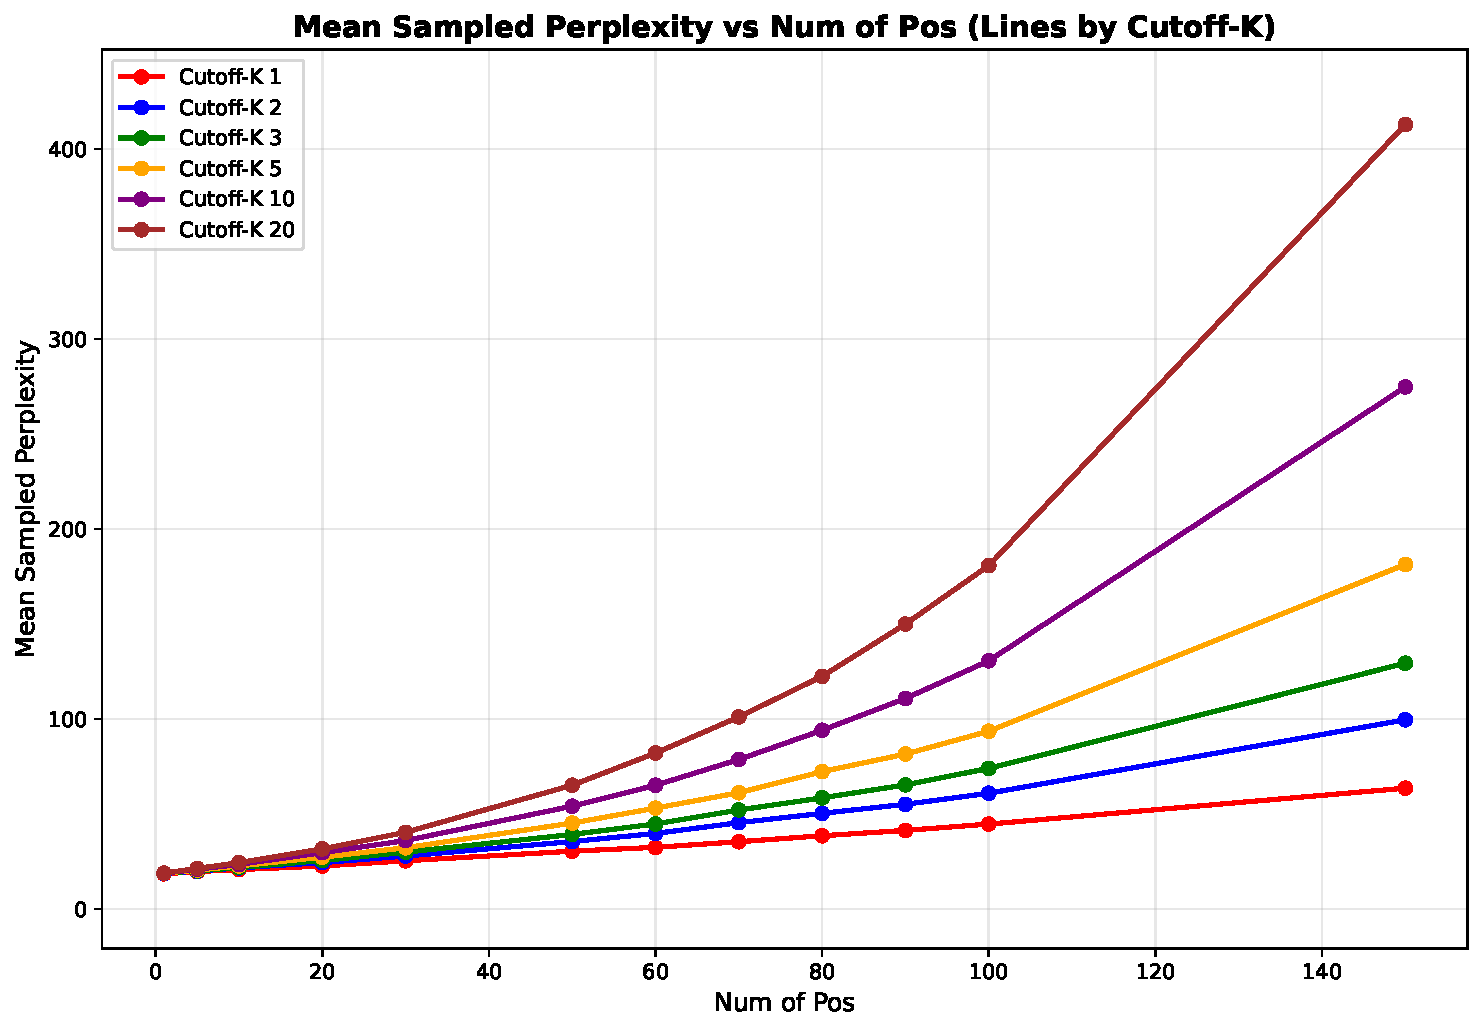
\includegraphics[width=0.45\textwidth]{graphs/attack/perplexity_main.pdf} % scale as needed
    \caption{Mean sampled perplexity vs number of perturbations made. Presented per each cutoff tested. The trend follows inverse curve to the model performance. Measured on facebook/opt-125m~\cite{facebook125m}.}
    \label{fig:perplexity}
\end{figure}

\begin{figure}[H]
    \centering
    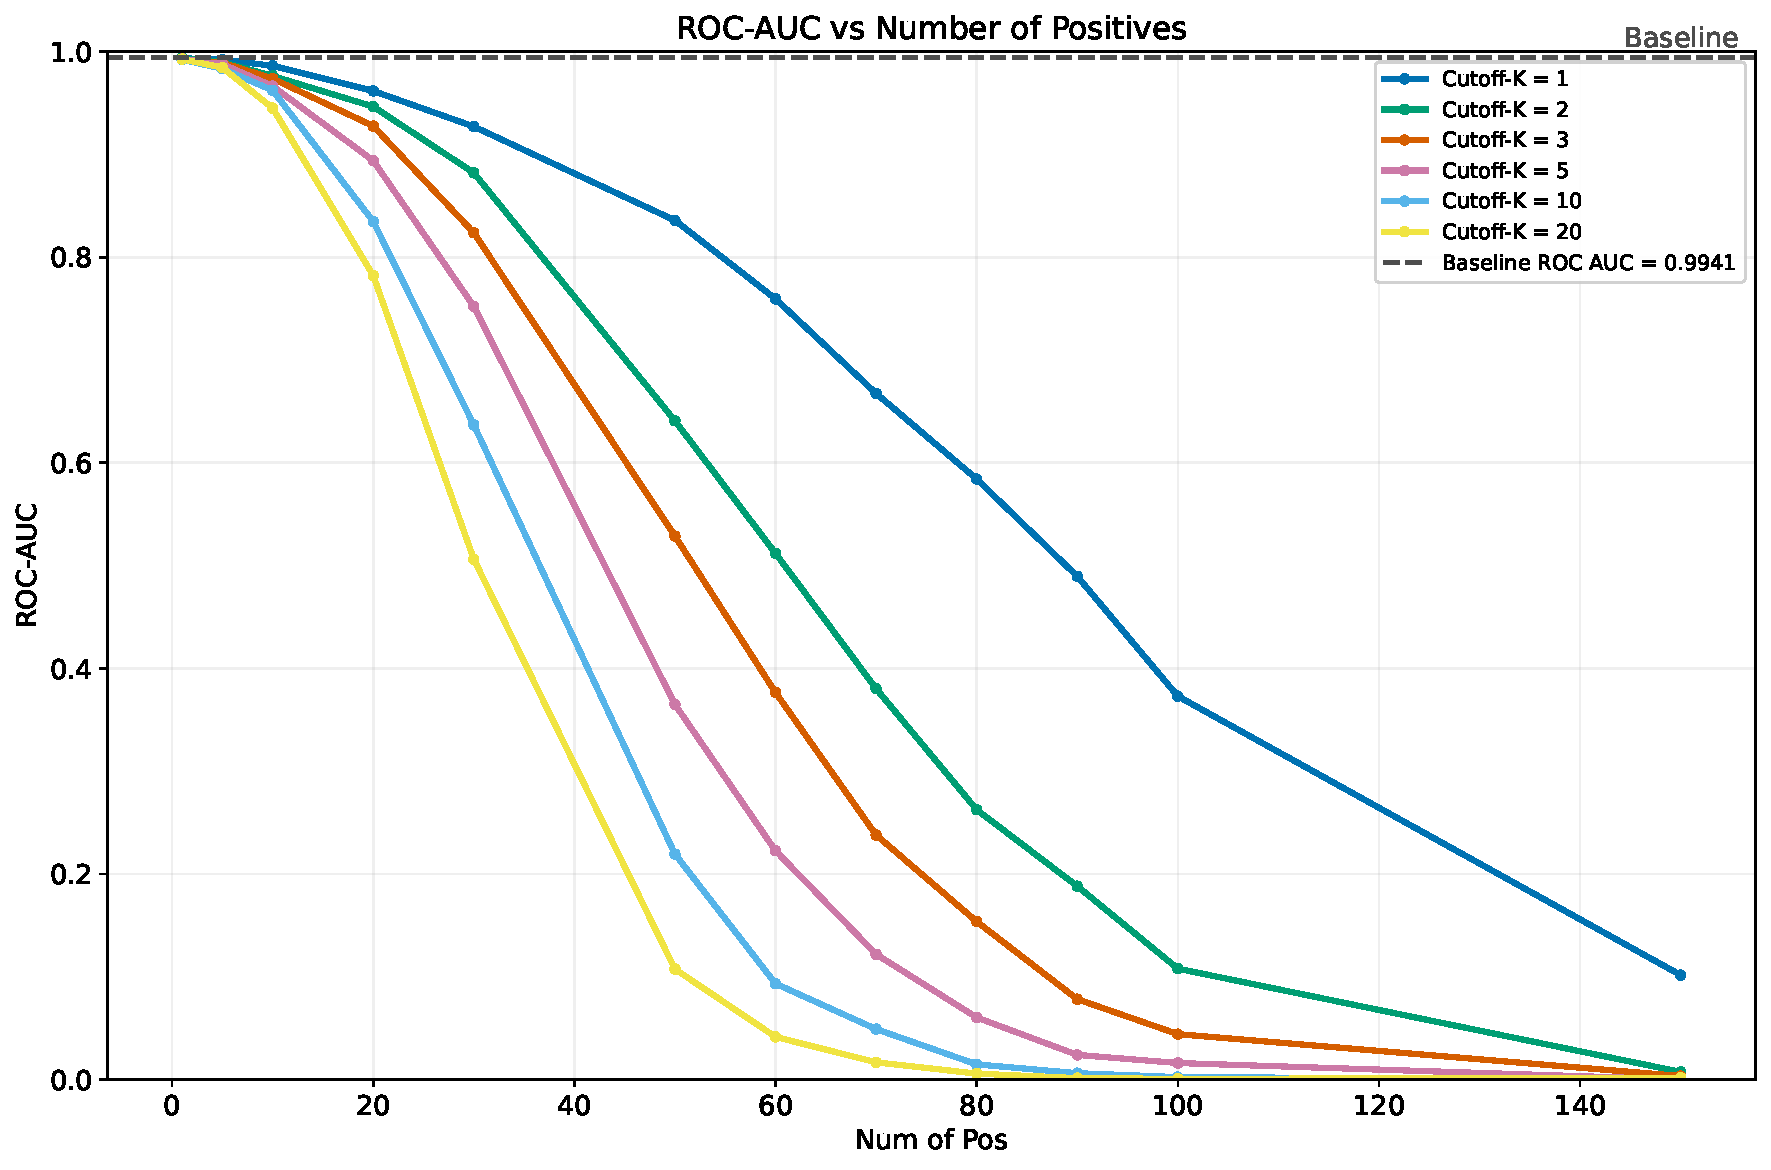
\includegraphics[width=0.45\textwidth]{graphs/attack/roc_vs_pos_by_k.pdf} % scale as needed
    \caption{ROC AUC vs number of perturbed positions, shown separately for different cutoff values. The dashed line indicates baseline performance without perturbation. ROC AUC decreases as the number of perturbations increases, with larger cutoffs accelerating the degradation. Results are reported for GPT-2 (124M)~\cite{radford2019language}.}
    \label{fig:ROC_attack}
\end{figure}

\begin{table}[H]
    \caption{Example texts under Mid-K attack with GPT-2 (124M) on XSum.}
    \label{tab:placeholder}
\vspace{1em}
\noindent
\textbf{Perturbation Results:}
\\
\begin{tabular}{|p{0.2\linewidth}|p{0.75\linewidth}|}
    \hline
    \textbf{Pos / Limit} & \textbf{Text} \\
    \hline
    Human & ``It was an oversight,'' Palmer told BBC Sport.\\
    \hline
    No perturbation & ``It was an honest and open challenge over the length of time,'' he said. \\
    \hline
    50 / 5 & ``It was an honest and open challenge over the length of time,'' he tells us.\\
    \hline
    150 / 1 & ``It was an honest and open challenge over exactly how this particular scheme could have become so costly to operate after it closed in 2001, we still do to this present day,'' said the report said\\
    \hline
    150 / 20 & ``It was an inappropriate response by the HL [Herodoplyosis Unit to complain that player Eddie Gabboni ran red before half goal]; in such situations players wear distinctive black shorts (most usually found throughout tournaments by Uprod on other social programs at venues as in RTS).\\
    \hline
\end{tabular}
\end{table}

\section{Algorithms}

\begin{algorithm*}[h]
  \caption{Fast-DetectGPT machine-generated text detection.}
  \textbf{Input:} passage $x$, sampling model $q_\varphi$, scoring model $p_\theta$, and decision threshold $\epsilon$ \\
  \textbf{Output:} True -- probably machine-generated, False -- probably human-written.
  \begin{algorithmic}[1]
    \label{alg:fastdetectgpt}
\Function{FastDetectGPT}{$x, q_\varphi, p_\theta$}
    \State $\tilde{x}_i \sim q_\varphi(\tilde{x}|x), i \in [1..N]$ \hfill $\triangleright$ Conditional sampling
    \State $\tilde{\mu} \leftarrow \frac{1}{N} \sum_i \log p_\theta(\tilde{x}_i|x)$ \hfill $\triangleright$ Estimate the mean
    \State $\tilde{\sigma}^2 \leftarrow \frac{1}{N-1} \sum_i (\log p_\theta(\tilde{x}_i|x) - \tilde{\mu})^2$ \hfill $\triangleright$ Estimate the variance
    \State $\hat{\mathrm{d}}_x \leftarrow (\log p_\theta(x) - \tilde{\mu})/\tilde{\sigma}$ \hfill $\triangleright$ Estimate conditional probability curvature
    \State \Return $\hat{\mathrm{d}}_x > \epsilon$ \hfill $\triangleright$ Compare with threshold
\EndFunction
\end{algorithmic}
\end{algorithm*}

\begin{algorithm*}[h]
  \caption{DetectGPT machine-generated text detection}
  \begin{algorithmic}[1]
    \label{alg:detectgpt}
\State \textbf{Input:} passage $x$, source model $p_\theta$, perturbation function $q$, number of perturbations $k$, decision threshold $\epsilon$
\State $\tilde{x}_i \sim q(\cdot \mid x)$, $i \in [1..k]$ \hfill $\triangleright$ mask spans, sample replacements
\State $\hat{\mu} \leftarrow \frac{1}{k} \sum_i \log p_\theta(\tilde{x}_i)$ \hfill $\triangleright$ approximate expectation in Eq. 1
\State $\hat{\mathrm{d}}_x \leftarrow \log p_\theta(x) - \hat{\mu}$ \hfill $\triangleright$ estimate d $(x, p_\theta, q)$
\State $\tilde{\sigma}_x^2 \leftarrow \frac{1}{k-1} \sum_i (\log p_\theta(\tilde{x}_i) - \hat{\mu})^2$ \hfill $\triangleright$ variance for normalization
\State \textbf{if} $\frac{\hat{\mathrm{d}}_x}{\tilde{\sigma}_x} > \epsilon$ \textbf{then}
\State \quad return \texttt{true} \hfill $\triangleright$ probably model sample
\State \textbf{else}
\State \quad return \texttt{false} \hfill $\triangleright$ probably not model sample
\end{algorithmic}
\end{algorithm*}



\newpage

% Bibliography entries for the entire Anthology, followed by custom entries
%\bibliography{anthology,custom}
% Custom bibliography entries only
\bibliography{custom}

\end{document}